\documentclass[11pt]{report}
\usepackage{tocloft}
\usepackage{sectsty}
%\usepackage{fullpage}
\usepackage[hidelinks]{hyperref}
\usepackage[utf8]{inputenc}
\usepackage{pdfpages}
\usepackage{multicol}
\usepackage{tabularx}

\renewcommand{\cftchapleader}{\cftdotfill{\cftdotsep}}
\renewcommand{\cftchapfont}{\normalfont}
\renewcommand{\cftchapaftersnum}{}
\renewcommand{\cftchappresnum}{Team\space}
\setlength{\cftchapnumwidth}{\widthof{\textbf{Team~99}}}

\renewcommand{\abstractname}{PREFACE}

\begin{document}

\newcommand{\mtopi}{$\textit{Math}^\textit{Industry}$~}
\newcommand{\person}[2]{\textbf{#1}, #2}
\sectionfont{\centering\sc\MakeLowercase}

% Front page is a PDF made via GIMP
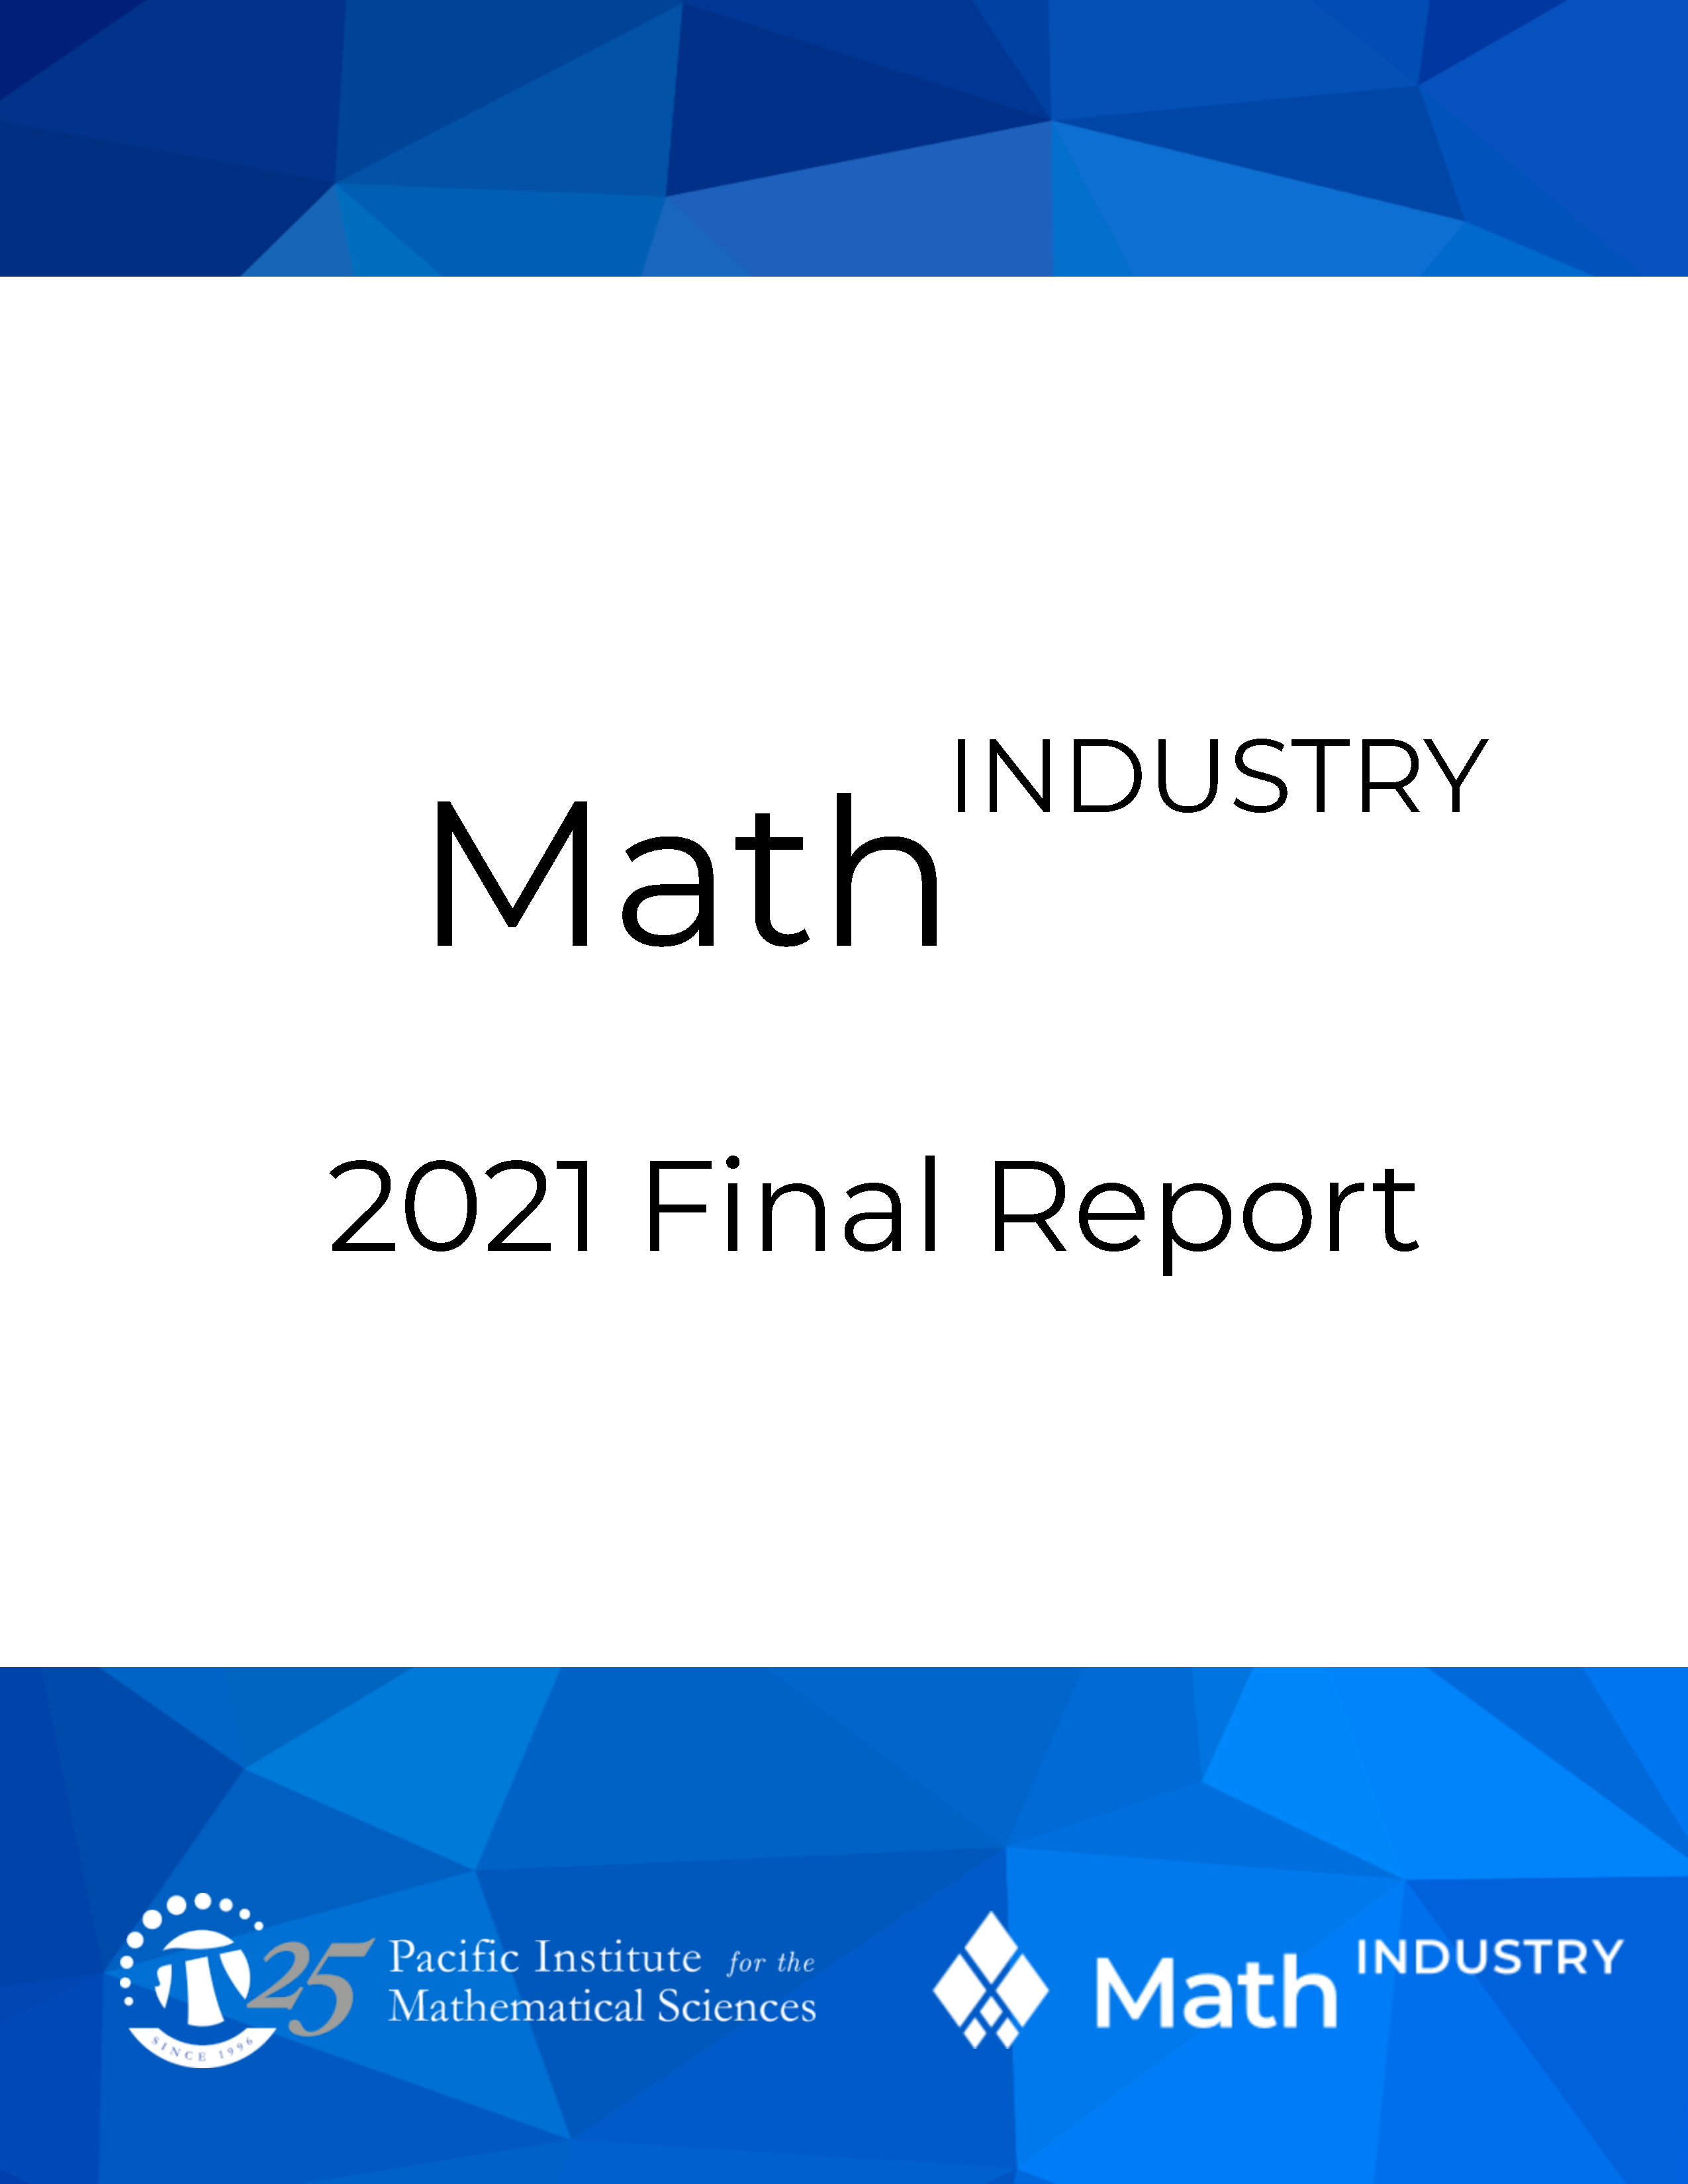
\includepdf[pages=1]{front-page.pdf}

\section*{Preface}
The second annual \mtopi (Math to Power Industry) virtual workshop took place
during August 2021, offered by the Pacific Institute for the Mathematical
Sciences (PIMS), with the help of its training and industrial partners.  The
workshop was launched in 2020 by PIMS in response to the economic impacts of
the COVID-19 pandemic on mathematical sciences graduates.  With the pandemic
impacts continuing in 2021, and an ever-increasing need for mathematics and
data sciences-skilled talent in North American industry sectors, online
workshops like this one have become a vital bridge for connecting mathematics
graduates and postdoctoral fellows to job opportunities in industry.

As in the first year, the workshop program began with a 10-day training
bootcamp followed by a 2-week experience working as part of a team on a real
problem provided by an industry or government agency partner.  Workshop
training courses included training on the latest programming and data workflow
environments, effective teamwork, EDI (equity, diversity, and inclusion),
communication, ethics in data science, startups and entrepreneurship.  Seven of
the real-world problems were contributed by industry partners, with four
companies returning from the previous year, and three were contributed by
municipal and federal government agencies.  Motivation for these problems
ranged from companies trying to make use artificial intelligence in their
decision-making, improve the safety and operation of their products, minimize
environmental impacts of food production and transport, manage and control
insect infestations, and improve the health of our communities.  Our teams
approached these problems through advanced mathematical modelling, statistics,
optimization, and computational techniques.  In some cases the results had
immediate positive impacts for these organizations, saving them both time and
money, and in other cases the industry partner or government agency was able to
use the workshop to recruit the highly skilled talent they need to be
successful.  

This \mtopi 2021 Final Report compiles the results obtained by each of the ten
workshop teams on their industry challenge.   


\newpage

\section*{Acknowledgements}
We acknowledge the contributions and participation of everyone that helped make
this event possible.  A heartfelt thank you to: 


\noindent\hrulefill

\begin{multicols}{2}
    \begin{flushleft}
        \uppercase{Aerium Analytics Ltd.} \\
        \uppercase{ATCO Ltd.} \\
        \uppercase{CSTS Health Care Ltd.} \\
        \uppercase{City of Winnipeg -- Insect Control Branch} \\
        \uppercase{IOTO International Ltd.} \\
        \uppercase{McMillan-McGee Ltd.} \\
        \uppercase{Natural Resources Canada} \\
        \uppercase{Serious Labs, Inc.} \\
        \uppercase{TheoryMesh Inc.}
    \end{flushleft}
 \end{multicols}

\noindent\hrulefill

We gratefully acknowledge the following people for providing mentorship or
other support to \mtopi teams. Their particular contributions are acknowledged
in the reports.

\noindent\hrulefill

\section*{Workshop Founders}
\begin{multicols}{2}
    \begin{flushleft} 
        \person{Dr. James Colliander}{former Director of PIMS} \\
        \columnbreak
        \person{Dr. Kristine Bauer}{UCalgary PIMS Site Director and PIMS Jobs Committee Chair}
    \end{flushleft}
\end{multicols}


\section*{ORGANIZING COMMITTEE}

\begin{multicols}{2}
    \begin{flushleft} 
        \person{Dr. Allen Herman}{URegina PIMS Site Director} \\
        \person{Dr. Matthew Greenberg}{UCalgary} \\
        \person{Dr. Jolen Gallagher}{Industrial Relations - UManitoba} \\
        \columnbreak
        \person{Dr. Linglong Kong}{UAlberta} \\
        \person{Ruth Situma}{PIMS Program and Communications Manager} \\
    \end{flushleft}
\end{multicols}


\begin{center} INSTRUCTORS \end{center}

\begin{multicols}{2}
    \begin{flushleft} 
        \person{Name 1}{Affiliation 1}

        \person{Name 2}{Affiliation 2}

        \person{Name 3}{Affiliation 3}

        \person{Name 4}{Affiliation 4}
    \end{flushleft}
\end{multicols}

\newpage

\begin{center} PARTICIPANT LIST \end{center}

\begin{multicols}{2}
    \begin{flushleft} 
        Name 1

        Name 2

        Name 3

        Name 4
    \end{flushleft}
\end{multicols}

\newpage

\tableofcontents

% Complete one \includepdf block for each project
\includepdf[
  pages=-,
  addtotoc={
    1,
    chapter,
    1,
    {{Author 1,
      Author 2
     }
     \textit{Project Title} \newline
     Company Name
    },
    teamXX
  }]{originals/team1.pdf}


\end{document}
